%Reference: http://www.theconstructionindex.co.uk/news/view/pay-now-argue-later
\subsection{Working Persona}
\label{sub:working_persona}

\marginpar{%
	\null
	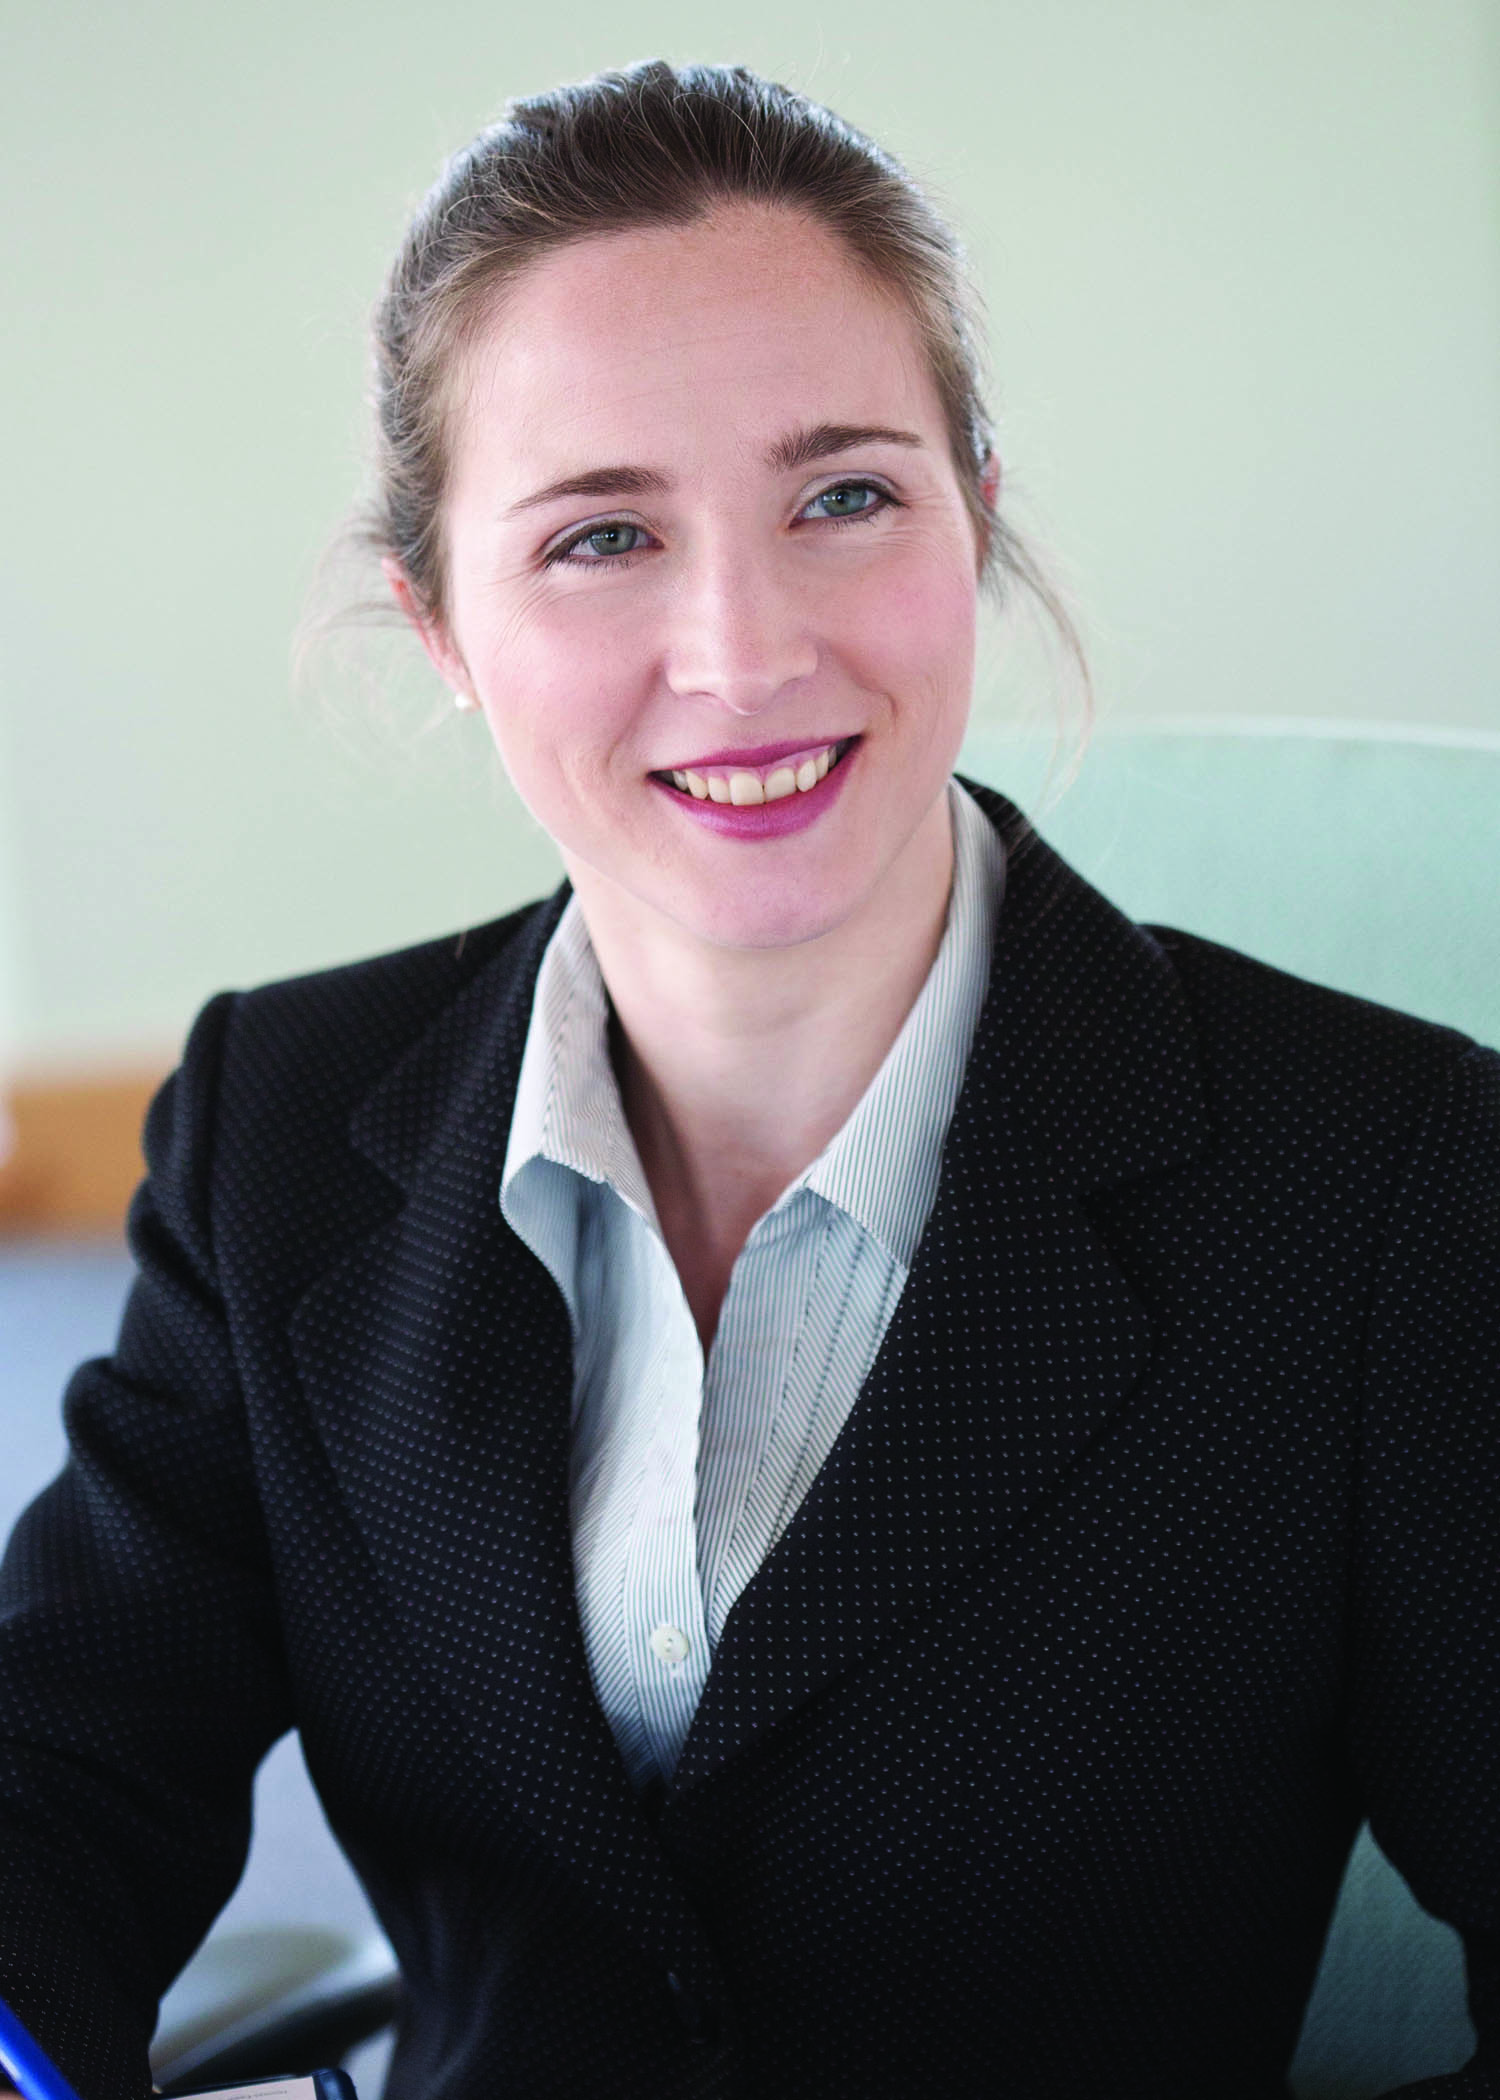
\includegraphics[width=\marginparwidth]{img/personas/working.jpg}
	\medskip
	\begin{description}[leftmargin=3cm]
		\item[Name] Janet
		\item[Occupation] IT Consultant
		\item[Age] 33
	\end{description}

	\subsection*{Main Goals}
	\begin{itemize}[leftmargin=1em]
		\item To play sport on her way home from work and at weekends
		\item To ease the stress of work and recent break-up
		\item Get involved in group sports to meet new people
	\end{itemize}
}

\subsubsection*{Description}
\label{ssub:working_description}

Janet lives in a flat in Sheffield but must commute to Leeds during the week
for work. Her job as an IT consultant  can be stressful and very time consuming
and often requires working late into the evenings. Due to her busy work
schedule, Janet is restricted to playing sport on occasional evenings and at
weekends. She doesn't have any children and currently lives on her own after
recently coming out of a long term relationship. And for that reason, she wants
to get out of the flat as much as possible and take her mind off things by
staying busy and active.

Janet wants to play sport on her drive home from work as she does not have time
to go home first. The fact she has a reasonably long commute gives Janet a
large area in which she can play sport, and therefore a greater selection of
sport centres to choose from. Due to her successful career, Janet has a decent
income so is not restricted by budget and is willing to pay extra for playing
at peak times. Her eagerness to stay active and keep busy means she is very
much up for playing any sports, even if she has never played them before.

Although Janet works in the IT industry, her experience with using
applications on a smart phone is limited.

% subsubsection description (end)

\subsubsection*{Scenarios}
\label{ssub:working_scenarios}

\begin{itemize}
	\item Janet feels like playing a team sport on Friday, she doesn't mind
		what sport but doesn't fancy doing something on her own. She has two
		friends who would like to get involved but would be willing to join
		other groups. The friends live far away and when they are organising
		the event, they would like to be able to share the same screen to make
		finding a suitable booking easier.

	\item It's a Tuesday evening and Janet has a table tennis session booked
		for 7pm. She has just been called in to an urgent meeting at work and
		doesn't think she can make the timeslot she has booked. She would like
		to see if she can push her timeslot back an hour, if not she must
		cancel.

	\item Janet has checked the weather forecast for next Saturday and it is
		looking to be a beautiful day. She has a coffee date at 2pm so can play
		any time before then and would like to play a sport outside.
\end{itemize}

% subsubsection scenarios (end)

\subsubsection*{Pain Points}
\label{ssub:working_pain_points}

\begin{itemize}
	\item Unpredictable work schedule.
\end{itemize}

% subsubsection pain_points (end)
